\chapter{Anexo A}

El Anexo A recoge y explica los procesos de instalación y configuración de los diferentes sistemas operativos, programas y herramientas necesarios para la implementación del proyecto.

% Configuración de la visualización del código SW
\lstset{backgroundcolor=\color{verde_p}, language=bash, breaklines=true, basicstyle=\footnotesize, xleftmargin=25pt, framesep=8pt, numbersep=15pt}


\section{Instalación de Raspbian OS}\label{anexo:raspbian}

Raspbian es un sistema operativo orientado a Raspberry Pi por lo que existe multitud de documentación complementaria en la web oficial\cite{Raspberry:2019}

Antes de comenzar a instalar el sistema operativo en una tarjeta microSD, se debe comprobar que ésta reúne los requisitos para ser usada en esta aplicación. Uno de estos requisitos es que la capacidad de la tarjeta sea superior a 8GB. Sin embargo, el uso de tarjetas de un tamaño superior a 32GB hace que sea necesario formatear la tarjeta antes de instalar el sistema operativo. Esto es debido a que el formato de serie (exFAT) no es compatible con el bootloader de Raspberry Pi, por lo que se deberá aplicar el formato FAT16 o FAT32 previamente.

Las instrucciones están pensadas teniendo en cuenta que se posee un ordenador con sistema operativo Windows.

\begin{enumerate}
\item \textbf{Descargar el sistema operativo}

Se puede descargar la imagen desde la web de descargas de Raspberry Pi\footnote{\url{https://www.raspberrypi.org/downloads/raspbian/}}

\begin{figure}[tb]
\centering
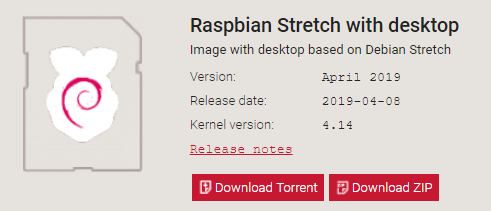
\includegraphics[width=0.5\textwidth]{figuras/RaspbianDwIcon.png}
\caption{Descarga de Raspbian Stretch}
\label{fig:descargaRaspbian}
\end{figure}

\item \textbf{Descargar e instalar Etcher}

Se precisa de una herramienta de escritura de imágenes y Etcher es la solución más sencilla para la mayoría de usuarios. Permite la escritura de la imagen sin la necesidad de extraer el archivo zip. 


\item \textbf{Escribir la imagen a una microSD}

Seleccionar el archivo de la imagen  la SD de destino es suficiente para flashear la imagen.

\item Una vez acabado el proceso de descompresión, la instalación debería estar completada. Introduciendo la tarjeta micro SD en su correspondiente posición en la Raspberry Pi, ésta acederá a Raspbian para arrancar el sistema.

\item Para comprobar la version del SO instalado, se puede hacer uso del comando \textit{lsb-release}

\begin{lstlisting}[frame=single, label=command:lsb]
lsb_release -a
\end{lstlisting}

\begin{figure}[tb]
\centering
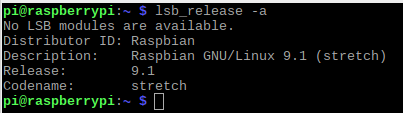
\includegraphics[width=0.5\textwidth]{figuras/RaspbianVersion.png}
\caption{Versión de Raspbian}
\label{fig:versionRaspbian}
\end{figure}

\end{enumerate}


\section{Instalación MQTT en Raspbian OS}\label{anexo:mqtt}

Mosquitto (broker de MQTT) se instala de igual manera que cualquier otra aplicación, haciendo uso de los repositorios.

En primer lugar, se actualizan los repositorios.

\begin{lstlisting}[frame=single, label=command:installmqtt1]
$ sudo apt-get update
\end{lstlisting}

Posteriormente, se instala Mosquitto.

\begin{lstlisting}[frame=single, label=command:installmqtt2]
$ sudo apt-get install mosquitto
\end{lstlisting}

Si todo va bien, al terminar el proceso, MQTT debería estar instalado.

Para probar la instalación, se pueden usar clientes de MQTT para enviar y recibir información a través un topic de prueba. Estos clientes son, por ejemplo, \textit{IoT MQTT Dashboard} en Android o \textit{MQTT.fx} en Windows.

\section{Edición y compilación de scripts en Raspbian OS}\label{anexo:scripts}

La edición de scripts y, en general, documentos de texto se realiza a través del programa \textit{gedit}. Es posible descargarlo e instalarlo a través del comando

\begin{lstlisting}[frame=single, label=command:installgedit]
$ sudo apt-get install gedit
\end{lstlisting} 

\textit{Gedit} es un editor de texto muy popular en sistemas basados en GNU/Linux, sencillo y ligero. Permite hacer poco más que editar el código con las herramientas más básicas, pero esto será suficiente. Se ejecuta con el comando siguiente, pero indicando el archivo que se quiere editar:

\begin{lstlisting}[frame=single, label=command:rungedit]
$ gedit /home/pi/Xbee/receive.py
\end{lstlisting} 

Los archivos con extensión \textit{.py} son scripts de Python que deben ser compilados y ejecutados. Para este cometido, existe un comando con el mismo nombre que el lenguaje. Para descargar Python, existe el siguiente comando\footnote{Se suponen los repositorios actualizados}:

\begin{lstlisting}[frame=single, label=command:installpython]
$ sudo apt install python2.7 python-pip
\end{lstlisting} 

Existen versiones posteriores de Python pero los scripts del presente proyecto han sido desarrollados de acuerdo a Python 2.7.13. Para comprobar si Python ya está instalado y su versión, se puede correr el siguiente comando:

\begin{lstlisting}[frame=single, label=command:checkpython]
$ python --version
Python 2.7.13
\end{lstlisting} 

Por último, a continuación se indica un ejemplo del comando usado para compilar y ejecutar un script en Linux (comando \ref{command:runpython}). Se deberá indicar el nombre del archivo que  al que queremos aplicar la acción.Si el script requiere de atributos de entrada, se deberán situar a continuación del nombre del archivo.

\begin{lstlisting}[frame=single, label=command:runpython]
$ sudo python /home/pi/Xbee/receive.py
\end{lstlisting} 

\chapter{Anexo B}\label{anexo:b}

En el Anexo B se sitúan los desarrollos software íntegros que forman parte del proyecto.

% Esto para configurar como se va a visualizar el código
\lstset{backgroundcolor=\color{amarillo_claro}, numbers=left,numberstyle=\tiny, language=Python, breaklines=true, basicstyle=\footnotesize, xleftmargin=25pt, framesep=8pt, numbersep=15pt}

\section{Código SendAT.py}\label{anexo:sendAT}

\begin{lstlisting}[frame=leftline, caption={SendAT.py}, label=code:SendAT]
#!/usr/bin/env python
import sys
import time
import serial
import logging

logging.basicConfig(filename='/home/pi/Xbee/SendLogs/sentAT.log',level=logging.DEBUG,format='%(asctime)s %(message)s')

ser = serial.Serial(
	port='/dev/ttyACM0',
	baudrate = 115200,
	parity=serial.PARITY_NONE,
	stopbits=serial.STOPBITS_ONE,
	bytesize=serial.EIGHTBITS,
	timeout=1
)

if len(sys.argv)<2:
	param = bytearray([0x8C,0x5A])
	logging.warning('AT Package non-defined values')
else:
	param = sys.argv[1]
	
val1 = param[0]+param[1]
val2 = param[3]+param[4]
var1 = int(val1,16)
var2 = int(val2,16)
checksum_rha = (~(6+2+var1+var2+125) & 0xFF)
	
if var1>124 and var1<167 and var2>59 and var2<111:
        values = bytearray([0xFF, 0xFF, 0x06, 0x02, 0x7D, var1, var2, checksum_rha])
        ser.write(values)
        logging.info('AT Package sent')
else:
        logging.warning('AT Package out of range')
    

\end{lstlisting}

\section{Código SendAPI.py}\label{anexo:sendAPI}

\begin{lstlisting}[frame=leftline, caption={SendAPI.py}, label=code:SendAPI]
#!/usr/bin/env python
import sys
import time
import serial
import logging

logging.basicConfig(filename='/home/pi/Xbee/SendLogs/sentAPI.log',level=logging.DEBUG,format='%(asctime)s %(message)s')

ser = serial.Serial(
	port='/dev/ttyACM0',
	baudrate = 115200,
	parity=serial.PARITY_NONE,
	stopbits=serial.STOPBITS_ONE,
	bytesize=serial.EIGHTBITS,
	timeout=1
)

if len(sys.argv)<2:
	param = bytearray([0x8C,0x5A])
	logging.warning('API Package non-defined values')
else:
	param = sys.argv[1]
	
val1 = param[0]+param[1]
val2 = param[3]+param[4]
var1 = int(val1,16)
var2 = int(val2,16)

checksum_rha = (~(6+2+var1+var2+125) & 0xFF)
checksum_xbee = (~(16+1+5*255+254+6+2+var1+var2+125+checksum_rha) & 0xFF)

if var1>124 and var1<167 and var2>59 and var2<111:
        values = bytearray([0x7E, 0x00, 0x16, 0x10, 0x01, 0x00, 0x00, 0x00, 0x00, 0x00, 0x00, 0xFF, 0xFF, 0xFF, 0xFE, 0x00, 0x00, 0xFF, 0xFF, 0x06, 0x02, 0x7D, var1, var2, checksum_rha, checksum_xbee])

        ser.write(values)
        logging.info('API Package sent')
        
else:
        logging.warning('API Package out of range')
\end{lstlisting}

\section{Código Receive.py}\label{anexo:receive}

\begin{lstlisting}[frame=leftline, caption={Receive.py}, label=code:Receive]
#!/usr/bin/env python
import sys
import time
import serial
import struct
import logging

logging.basicConfig(filename='/home/pi/Xbee/ReceiveLogs/receiveAT.log',level=logging.DEBUG,format='%(asctime)s %(message)s')

ser = serial.Serial(
	port='/dev/ttyACM0',
	baudrate = 115200,
	parity=serial.PARITY_NONE,
	stopbits=serial.STOPBITS_ONE,
	bytesize=serial.EIGHTBITS,
	timeout=1
)

def serialReader():
    b = ser.read()
    if b:
        bs = struct.unpack("<B",b)
        return int(bs[0])
    else:
        return -1

while True:
        if serialReader() == 255 and serialReader() == 255:
            length = serialReader()
            data = [0]*length
            for x in xrange(length):
                data[x] = serialReader()
            if data[0] == 0: # 0 means an UPDATE_INFO package
                dev = [data[6],data[11]]
                logging.info(data)
                print(dev,file=sys.stderr)
                
\end{lstlisting}

\chapter{Anexo C}

El Anexo C recoge la documentación de interés de distintos componentes del proyecto

\section{Documentación de XBee Shield}\label{anexo:XBShield}

\begin{figure}[H]
\centering
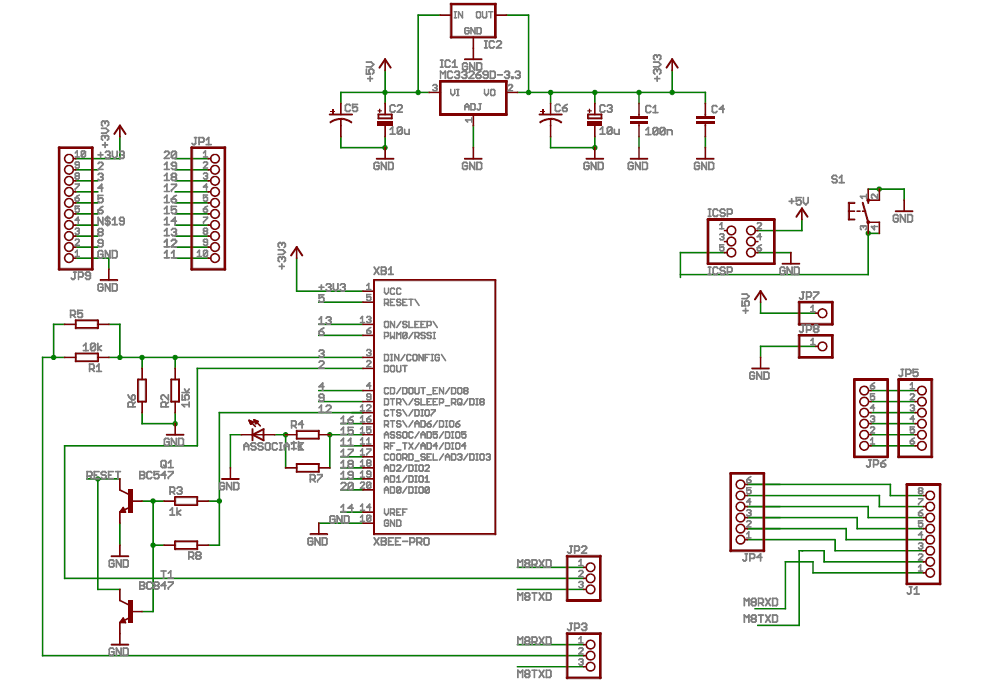
\includegraphics[width=1\textwidth]{figuras/XbeeShSch.png}
\caption{Esquemático de XBee Shield}
\label{fig:esquemaXBShield}
\end{figure}

\section{Pruebas del proyecto}\label{anexo:test}

\begin{figure}[H]
\centering
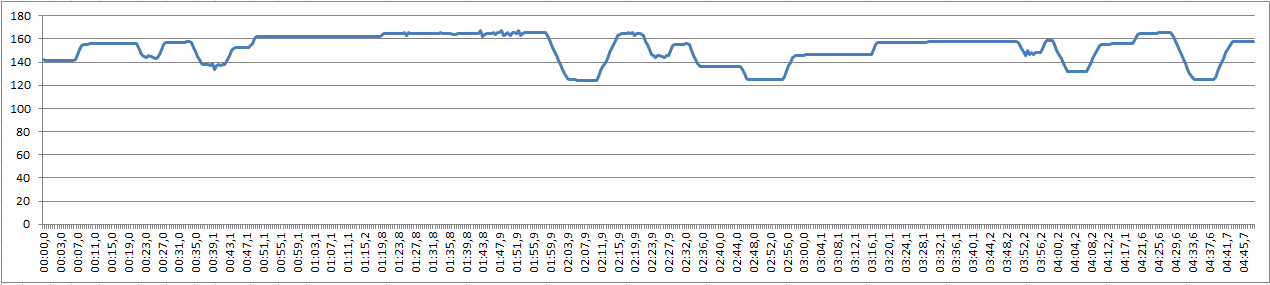
\includegraphics[width=1.1\textwidth]{figuras/trec1.png}
\caption{Test de recepción de datos AT}
\end{figure}

\begin{figure}[H]
\centering
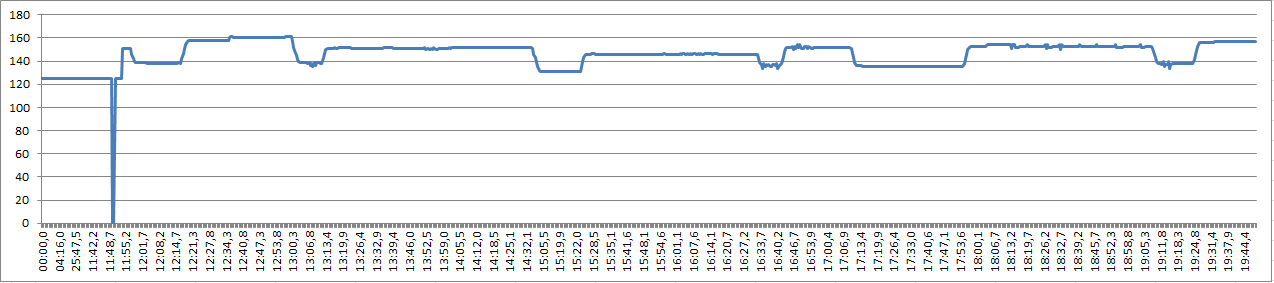
\includegraphics[width=1.1\textwidth]{figuras/trec2.png}
\caption{Test de recepción de datos genérico 1}
\end{figure}

\begin{figure}[H]
\centering
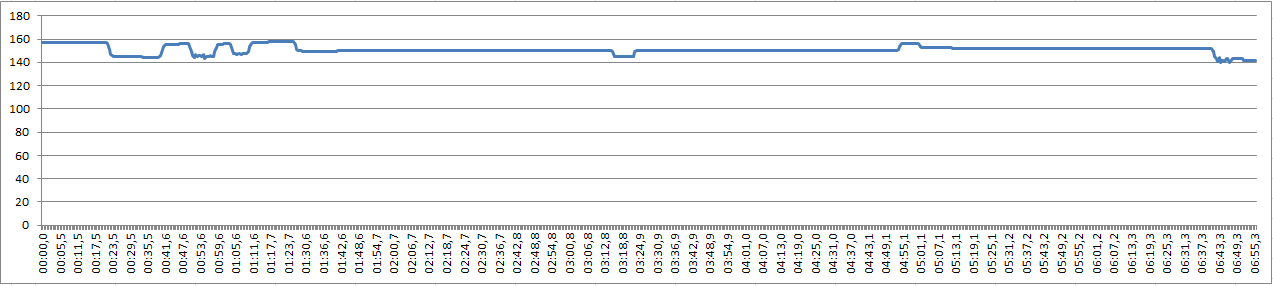
\includegraphics[width=1.1\textwidth]{figuras/trec4.png}
\caption{Test de recepción de datos genérico 2}
\end{figure}

\begin{figure}[H]
\centering
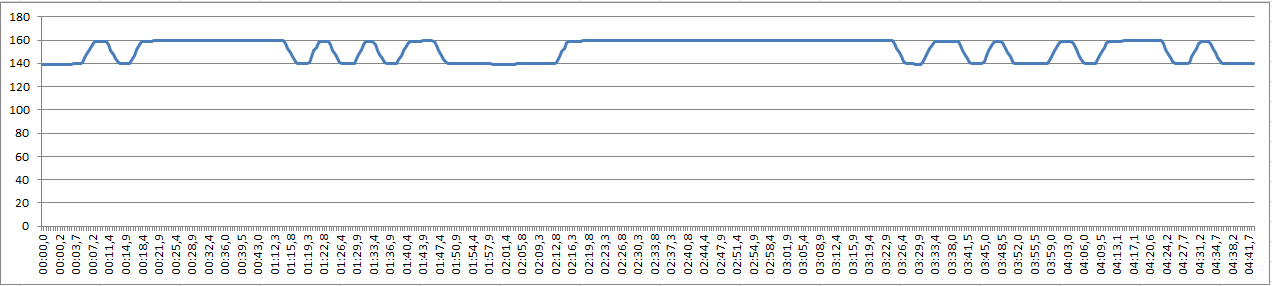
\includegraphics[width=1.1\textwidth]{figuras/trec3.png}
\caption{Test de recepción de datos MQTT}
\end{figure}

\begin{figure}[H]
\centering
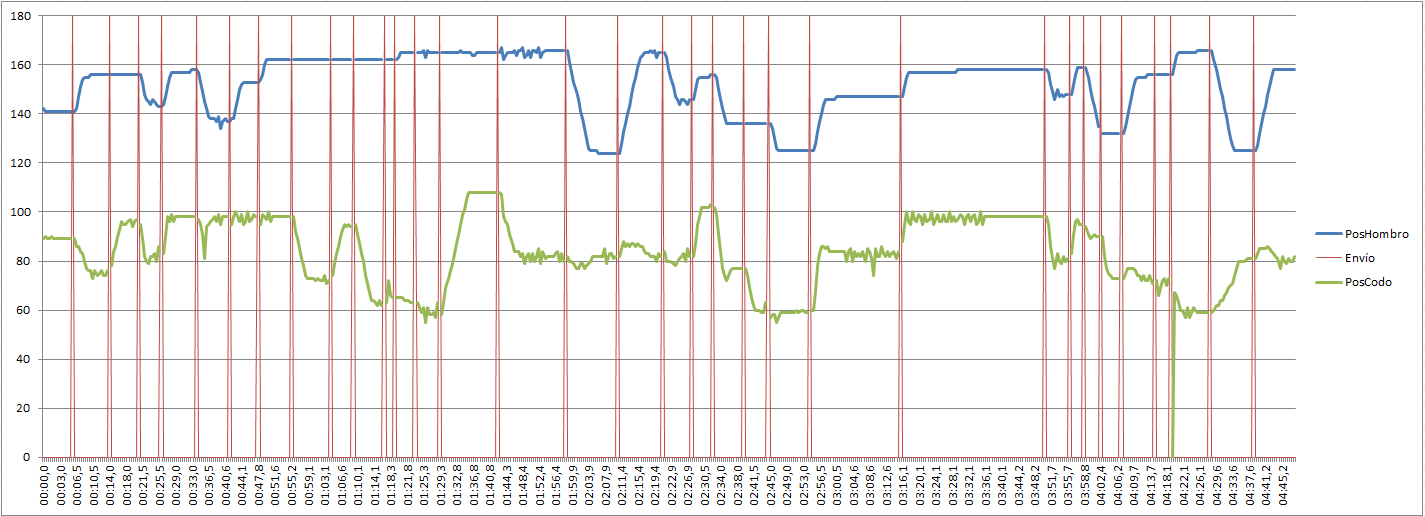
\includegraphics[width=1.1\textwidth]{figuras/temat.png}
\caption{Test de emisión AT de datos}
\end{figure}

\begin{figure}[H]
\centering
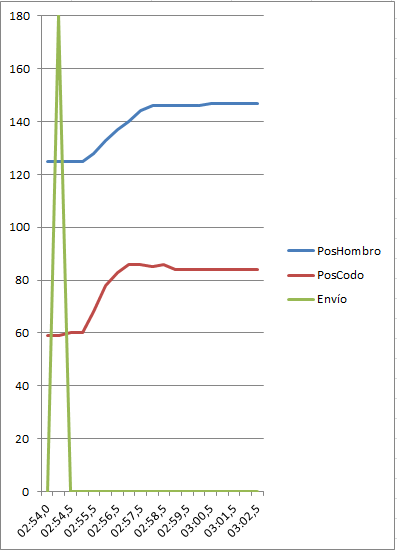
\includegraphics[width=0.4\textwidth]{figuras/tresp.png}
\caption{Detalle de la respuesta ante un paquete de mando}
\end{figure}

\begin{table}[H]
\begin{center}
\begin{tabular}{|m{15mm}|m{15mm}||m{15mm}|m{15mm}||m{15mm}|m{15mm}||m{15mm}|m{15mm}|}
\hline
\textbf{Muestra} & \textbf{Tiempo} & \textbf{Muestra} & \textbf{Tiempo} & \textbf{Muestra} & \textbf{Tiempo} & \textbf{Muestra} & \textbf{Tiempo}\\
\hline
1 & 0.767 & 9 & 0.295 & 17 & 0.667 & 25 & 0.686\\
\hline
2 & 0.48 & 10 & 0.852 & 18 & 0.885 & 26 & 0.908\\
\hline
3 & 0.822 & 11 & 0.896 & 19 & 0.702 & 27 & 0.76\\
\hline
4 & 0.261 & 12 & 0.909 & 20 & 0.658 & 28 & 0.962\\
\hline
5 & 0.487 & 13 & 0.524 & 21 & 0.576 & 29 & 1.001\\
\hline
6 & 0.544 & 14 & 0.524 & 22 & 1.037 & 30 & 0.895\\
\hline
7 & 0.793 & 15 & 0.931 & 23 & 0.482 & 31 & 0.889\\
\hline
8 & 0.942 & 16 & 0.925 & 24 & 0.648 & - & -\\
\hline
\end{tabular}
\end{center}
\caption{Tiempos de reacción ante el envío de datos}
\label{tab:treac}
\end{table}

\begin{figure}[H]
\centering
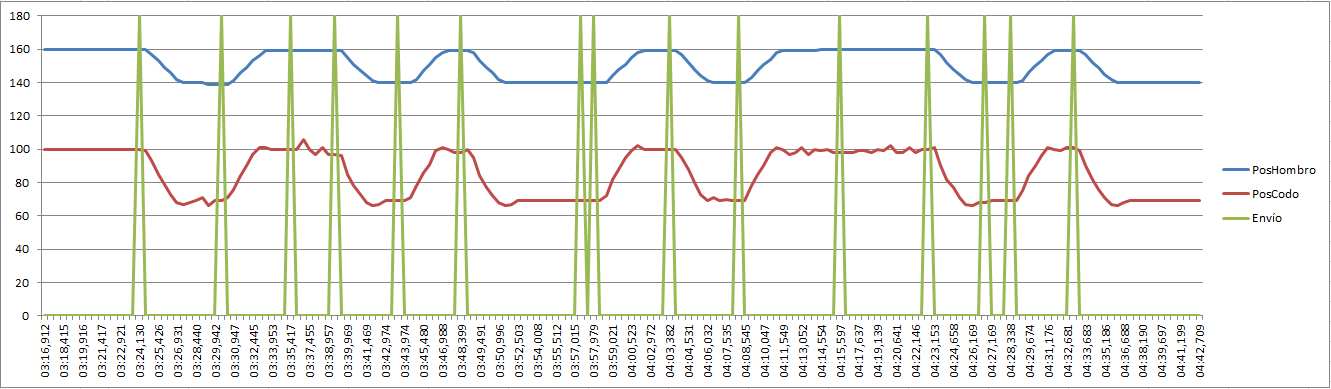
\includegraphics[width=1.1\textwidth]{figuras/tmqtt.png}
\caption{Test de uso MQTT}
\end{figure}
